\PassOptionsToPackage{unicode}{hyperref}
\PassOptionsToPackage{hyphens}{url}
\PassOptionsToPackage{dvipsnames,svgnames,x11names}{xcolor}
\documentclass[
  spanish,
  11pt,
  a4paper,
  DIV=11,
  numbers=noendperiod]{scrartcl}

\usepackage{xcolor}
\usepackage[top=24mm,bottom=24mm,left=24mm,right=24mm,headheight=15pt,headsep=8mm]{geometry}
\usepackage{amsmath,amssymb}
\usepackage{iftex}
\ifPDFTeX
  \usepackage[T1]{fontenc}
  \usepackage[utf8]{inputenc}
  \usepackage{textcomp}
\else
  \usepackage{unicode-math}
  \defaultfontfeatures{Scale=MatchLowercase}
  \defaultfontfeatures[\rmfamily]{Ligatures=TeX,Scale=1}
\fi
\usepackage{lmodern}
\IfFileExists{upquote.sty}{\usepackage{upquote}}{}
\IfFileExists{microtype.sty}{
  \usepackage[]{microtype}
  \UseMicrotypeSet[protrusion]{basicmath}
}{}
\usepackage{graphicx}
\usepackage{float}
\usepackage[bidi=basic]{babel}
\let\LanguageShortHands\languageshorthands
\def\languageshorthands#1{}
\setlength{\emergencystretch}{3em}
\setcounter{secnumdepth}{5}
\providecommand{\tightlist}{\setlength{\itemsep}{0pt}\setlength{\parskip}{0pt}}

\newcommand{\practicaPdfCoverImage}{}
% PDF style for Practica 9.
% A modest university handout look: classical type, clear hierarchy,
% restrained color, and durable code/callout styling.

\usepackage{graphicx}
\usepackage[export]{adjustbox}
\usepackage{fontspec}
\usepackage{microtype}
\usepackage{scrlayer-scrpage}
\usepackage{tikz}
\usepackage{fvextra}
\usepackage{caption}
\usepackage{subcaption}
\usepackage[skins,breakable]{tcolorbox}

\providecommand{\practicaPdfCoverImage}{}

\definecolor{uzaInk}{HTML}{172033}
\definecolor{uzaMuted}{HTML}{5F6B7A}
\definecolor{uzaBlue}{HTML}{1F5F8B}
\definecolor{uzaBlueDark}{HTML}{153E5C}
\definecolor{uzaCyan}{HTML}{EAF4F7}
\definecolor{uzaLine}{HTML}{D7E2EA}
\definecolor{uzaCodeBg}{HTML}{F5F7F9}
\definecolor{uzaTip}{HTML}{237A57}
\definecolor{uzaWarn}{HTML}{A65F00}

\IfFontExistsTF{TeX Gyre Pagella}{
  \setmainfont{TeX Gyre Pagella}
}{}
\IfFontExistsTF{TeX Gyre Heros}{
  \setsansfont{TeX Gyre Heros}
}{}
\IfFontExistsTF{TeX Gyre Cursor}{
  \setmonofont{TeX Gyre Cursor}[Scale=0.86]
}{
  \setmonofont{Latin Modern Mono}[Scale=0.88]
}

\KOMAoptions{parskip=half}
\setlength{\parindent}{0pt}
\setlength{\parskip}{0.55em plus 0.15em minus 0.08em}
\linespread{1.035}

\addtokomafont{disposition}{\sffamily\color{uzaBlueDark}}
\addtokomafont{section}{\LARGE}
\addtokomafont{subsection}{\Large}
\addtokomafont{subsubsection}{\normalsize\bfseries}
\RedeclareSectionCommand[beforeskip=2.2em plus 0.4em minus 0.2em,afterskip=1.0em]{section}
\RedeclareSectionCommand[beforeskip=1.2em,afterskip=0.55em]{subsection}
\RedeclareSectionCommand[beforeskip=1.0em,afterskip=0.35em]{subsubsection}

\clearpairofpagestyles
\automark[section]{section}
\ihead{\sffamily\footnotesize\textcolor{uzaMuted}{Informática (30717)}}
\ohead{\sffamily\footnotesize\textcolor{uzaMuted}{\headmark}}
\cfoot{\sffamily\small\textcolor{uzaMuted}{\pagemark}}
\setkomafont{pageheadfoot}{\normalfont}
\KOMAoptions{headsepline=0.35pt}
\addtokomafont{headsepline}{\color{uzaLine}}

\makeatletter
\AtBeginDocument{%
  \hypersetup{
    linkcolor=uzaBlueDark,
    urlcolor=uzaBlue,
    citecolor=uzaBlueDark
  }%
  \@ifundefined{Highlighting}{%
    \DefineVerbatimEnvironment{Highlighting}{Verbatim}{
      commandchars=\\\{\},
      fontsize=\small,
      breaklines=true,
      breakanywhere=true
    }%
  }{%
    \RecustomVerbatimEnvironment{Highlighting}{Verbatim}{
      commandchars=\\\{\},
      fontsize=\small,
      breaklines=true,
      breakanywhere=true
    }%
  }%
  \@ifundefined{Shaded}{%
    \newenvironment{Shaded}{%
      \begin{tcolorbox}[
        enhanced,
        breakable,
        sharp corners,
        boxrule=0.25pt,
        colback=uzaCodeBg,
        colframe=uzaLine,
        borderline west={1.4pt}{0pt}{uzaBlue},
        left=2mm,
        right=2mm,
        top=1.4mm,
        bottom=1.4mm,
        before skip=0.75em,
        after skip=0.75em
      ]%
    }{%
      \end{tcolorbox}%
    }%
  }{%
    \renewenvironment{Shaded}{%
      \begin{tcolorbox}[
        enhanced,
        breakable,
        sharp corners,
        boxrule=0.25pt,
        colback=uzaCodeBg,
        colframe=uzaLine,
        borderline west={1.4pt}{0pt}{uzaBlue},
        left=2mm,
        right=2mm,
        top=1.4mm,
        bottom=1.4mm,
        before skip=0.75em,
        after skip=0.75em
      ]%
    }{%
      \end{tcolorbox}%
    }%
  }%
}
\makeatother

\newcommand{\PracticeCode}[1]{%
  \begin{Shaded}%
  \VerbatimInput[
    fontsize=\small,
    breaklines=true,
    breakanywhere=true
  ]{#1}%
  \end{Shaded}%
}

\makeatletter
\renewcommand{\maketitle}{%
  \begin{titlepage}
    \thispagestyle{empty}
    \begin{tikzpicture}[remember picture,overlay]
      \fill[uzaCyan] (current page.north west) rectangle ([yshift=-72mm]current page.north east);
      \fill[uzaBlue] (current page.north west) rectangle ([xshift=7mm]current page.south west);
    \end{tikzpicture}
    \vspace*{12mm}
    {\sffamily\small\bfseries\textcolor{uzaBlue}{INFORMÁTICA (30717)}}\par
    \vspace{5mm}
    {\sffamily\bfseries\fontsize{30}{35}\selectfont\textcolor{uzaInk}{\@title}}\par
    \vspace{3mm}
    {\sffamily\Large\textcolor{uzaMuted}{Grado en Estudios en Arquitectura}}\par
    \vspace{8mm}
    {\color{uzaBlue}\rule{\textwidth}{0.6pt}}\par
    \if\relax\detokenize\expandafter{\practicaPdfCoverImage}\relax
    \else
      \vspace{5mm}
      {\centering\includegraphics[width=\textwidth,height=78mm,keepaspectratio]{\practicaPdfCoverImage}\par}
    \fi
    \vfill
    {\sffamily\large\textcolor{uzaBlueDark}{Universidad de Zaragoza}}\par
    \vspace{2mm}
    {\sffamily\small\textcolor{uzaMuted}{Material de prácticas del curso 2025--2026}}\par
  \end{titlepage}
}
\makeatother

\captionsetup{
  font={small,sf},
  labelfont={bf,color=uzaBlueDark},
  textfont={color=uzaInk},
  justification=centering,
  singlelinecheck=false,
  skip=6pt
}
\captionsetup[subfigure]{
  font={small,sf},
  labelfont={bf,color=uzaBlueDark},
  justification=centering,
  singlelinecheck=true,
  skip=4pt
}

\newcommand{\PracticeCredit}[1]{\textcolor{uzaMuted}{#1}}
\newcommand{\PracticeImagePair}[6]{%
  \begin{figure}[tbp]
    \centering
    \begin{minipage}[t]{0.485\linewidth}
      \includegraphics[width=\linewidth]{#3}
      \vspace{2mm}
      \centering{\sffamily\footnotesize #4}
    \end{minipage}\hfill
    \begin{minipage}[t]{0.485\linewidth}
      \includegraphics[width=\linewidth]{#5}
      \vspace{2mm}
      \centering{\sffamily\footnotesize #6}
    \end{minipage}
    \caption{\label{#1}#2}
  \end{figure}
}

\renewcommand{\arraystretch}{1.16}
\setlength{\tabcolsep}{6pt}
\setkeys{Gin}{center}

% Quarto callout colors are referenced by generated tcolorbox options.
% Apply them at document start so they win over Quarto's defaults.
\AtBeginDocument{%
  \definecolor{quarto-callout-note-color}{HTML}{1F5F8B}%
  \definecolor{quarto-callout-note-color-frame}{HTML}{1F5F8B}%
  \definecolor{quarto-callout-tip-color}{HTML}{237A57}%
  \definecolor{quarto-callout-tip-color-frame}{HTML}{237A57}%
  \definecolor{quarto-callout-warning-color}{HTML}{A65F00}%
  \definecolor{quarto-callout-warning-color-frame}{HTML}{A65F00}%
  \definecolor{quarto-callout-important-color}{HTML}{9B2C2C}%
  \definecolor{quarto-callout-important-color-frame}{HTML}{9B2C2C}%
  \definecolor{quarto-callout-caution-color}{HTML}{B45309}%
  \definecolor{quarto-callout-caution-color-frame}{HTML}{B45309}%
}

\KOMAoption{captions}{tableheading}
\usetikzlibrary{arrows.meta}

\newtcolorbox{PracticeWarningBox}[1]{%
  enhanced,
  breakable,
  sharp corners,
  boxrule=0.25pt,
  colback=white,
  colframe=uzaLine,
  colbacktitle=uzaCyan,
  coltitle=uzaInk,
  fonttitle=\sffamily\bfseries,
  title={#1},
  borderline west={1.4pt}{0pt}{uzaWarn},
  left=2mm,
  right=2mm,
  top=1.4mm,
  bottom=1.4mm,
  before skip=0.75em,
  after skip=0.75em
}

\newtcolorbox{PracticeImportantBox}[1]{%
  enhanced,
  breakable,
  sharp corners,
  boxrule=0.25pt,
  colback=white,
  colframe=uzaLine,
  colbacktitle=uzaCyan,
  coltitle=uzaInk,
  fonttitle=\sffamily\bfseries,
  title={#1},
  borderline west={1.4pt}{0pt}{red!55!black},
  left=2mm,
  right=2mm,
  top=1.4mm,
  bottom=1.4mm,
  before skip=0.75em,
  after skip=0.75em
}

\usepackage{bookmark}
\IfFileExists{xurl.sty}{\usepackage{xurl}}{}
\urlstyle{same}
\hypersetup{
  pdftitle={Práctica 5: Resolución de problemas en Java (II)},
  pdflang={es},
  colorlinks=true,
  linkcolor={uzaBlueDark},
  filecolor={Maroon},
  citecolor={Blue},
  urlcolor={uzaBlue},
  pdfcreator={LaTeX}
}

\title{Práctica 5: Resolución de problemas en Java (II)}
\author{}
\date{}

\begin{document}
\maketitle

\renewcommand*\contentsname{Tabla de contenidos}
{
\hypersetup{linkcolor=}
\setcounter{tocdepth}{2}
\tableofcontents
}

\clearpage

\section{Objetivos de la práctica}\label{objetivos-de-la-practica}

Los objetivos de la quinta práctica de la asignatura son los siguientes:

\begin{itemize}
\tightlist
\item Desarrollar algoritmos en Java.
\item Ejecutar algoritmos en el entorno \emph{Eclipse}.
\end{itemize}

\section{Criba de Eratóstenes}\label{criba-de-eratostenes}

La \textbf{criba de Eratóstenes} es un algoritmo eficiente para \textbf{encontrar todos los números primos menores o iguales a un número dado}. El algoritmo funciona de la siguiente manera:

\begin{enumerate}
\tightlist
\item Se guardan en un vector todos los números desde 2 hasta el número dado.
\item Se comienza con el primer número primo, 2, y se descartan todos los múltiplos de ese número.
\item Se repite el proceso con el siguiente número primo en el vector hasta que se hayan procesado todos los números.
\end{enumerate}

Por ejemplo, para encontrar los números primos menores o iguales a 30, el algoritmo eliminaría los múltiplos de 2, luego los múltiplos de 3, y así sucesivamente, dejando solo los números primos \(2, 3, 5, 7, 11, 13, 17, 19, 23, 29\).

\section{Vectores en Java}\label{vectores-en-java}

A modo de recordatorio, un \textbf{vector en Java} es una colección de elementos del mismo tipo. Se puede declarar y utilizar un vector de números enteros de la siguiente manera:

\PracticeCode{../resources/practica5/snippets/java/vector-example.java}

\section{Ejercicios}\label{ejercicios}

La criba de Eratóstenes se puede implementar de varias maneras, dependiendo de cómo se manejen los datos y se optimice el proceso. A continuación se presentan cuatro posibles soluciones. Cada solución se deberá implementar en una clase separada, de nombre \texttt{Solucion1.java}, \texttt{Solucion2.java}, \texttt{Solucion3.java} y \texttt{Solucion4.java}, respectivamente.

El objetivo es modificar cada una de las implementaciones para \textbf{contar el número de tachones} que realiza cada una de las implementaciones de la criba, y \textbf{medir su tiempo de ejecución}.

\subsection{Tiempos de ejecución}\label{tiempos-de-ejecucion}

Anota el tiempo de ejecución en Microsoft Excel para cada una de las implementaciones, y cuatro valores de \(n\) diferentes: \(10^4\), \(10^5\), \(10^6\) y \(10^7\). Los valores de \(n\) se representarán en el eje \(X\) de un gráfico, y el tiempo de ejecución en el eje \(Y\).

\begin{table}[H]
\centering
\begin{tabular}{r|rrrr}
\textbf{\(n\)} & \textbf{Solución 1} & \textbf{Solución 2} & \textbf{Solución 3} & \textbf{Solución 4} \\
\hline
10\,000 & 21 & 21 & 19 & 18 \\
100\,000 & 52 & 55 & 52 & 43 \\
1\,000\,000 & 215 & 209 & 184 & 220 \\
10\,000\,000 & 1286 & 1106 & 1060 & 1012 \\
\end{tabular}
\caption{Tabla de tiempos de ejecución en milisegundos de las diferentes implementaciones de la criba de Eratóstenes.}\label{tbl-p5-tiempos}
\end{table}

\begin{figure}[H]
\centering
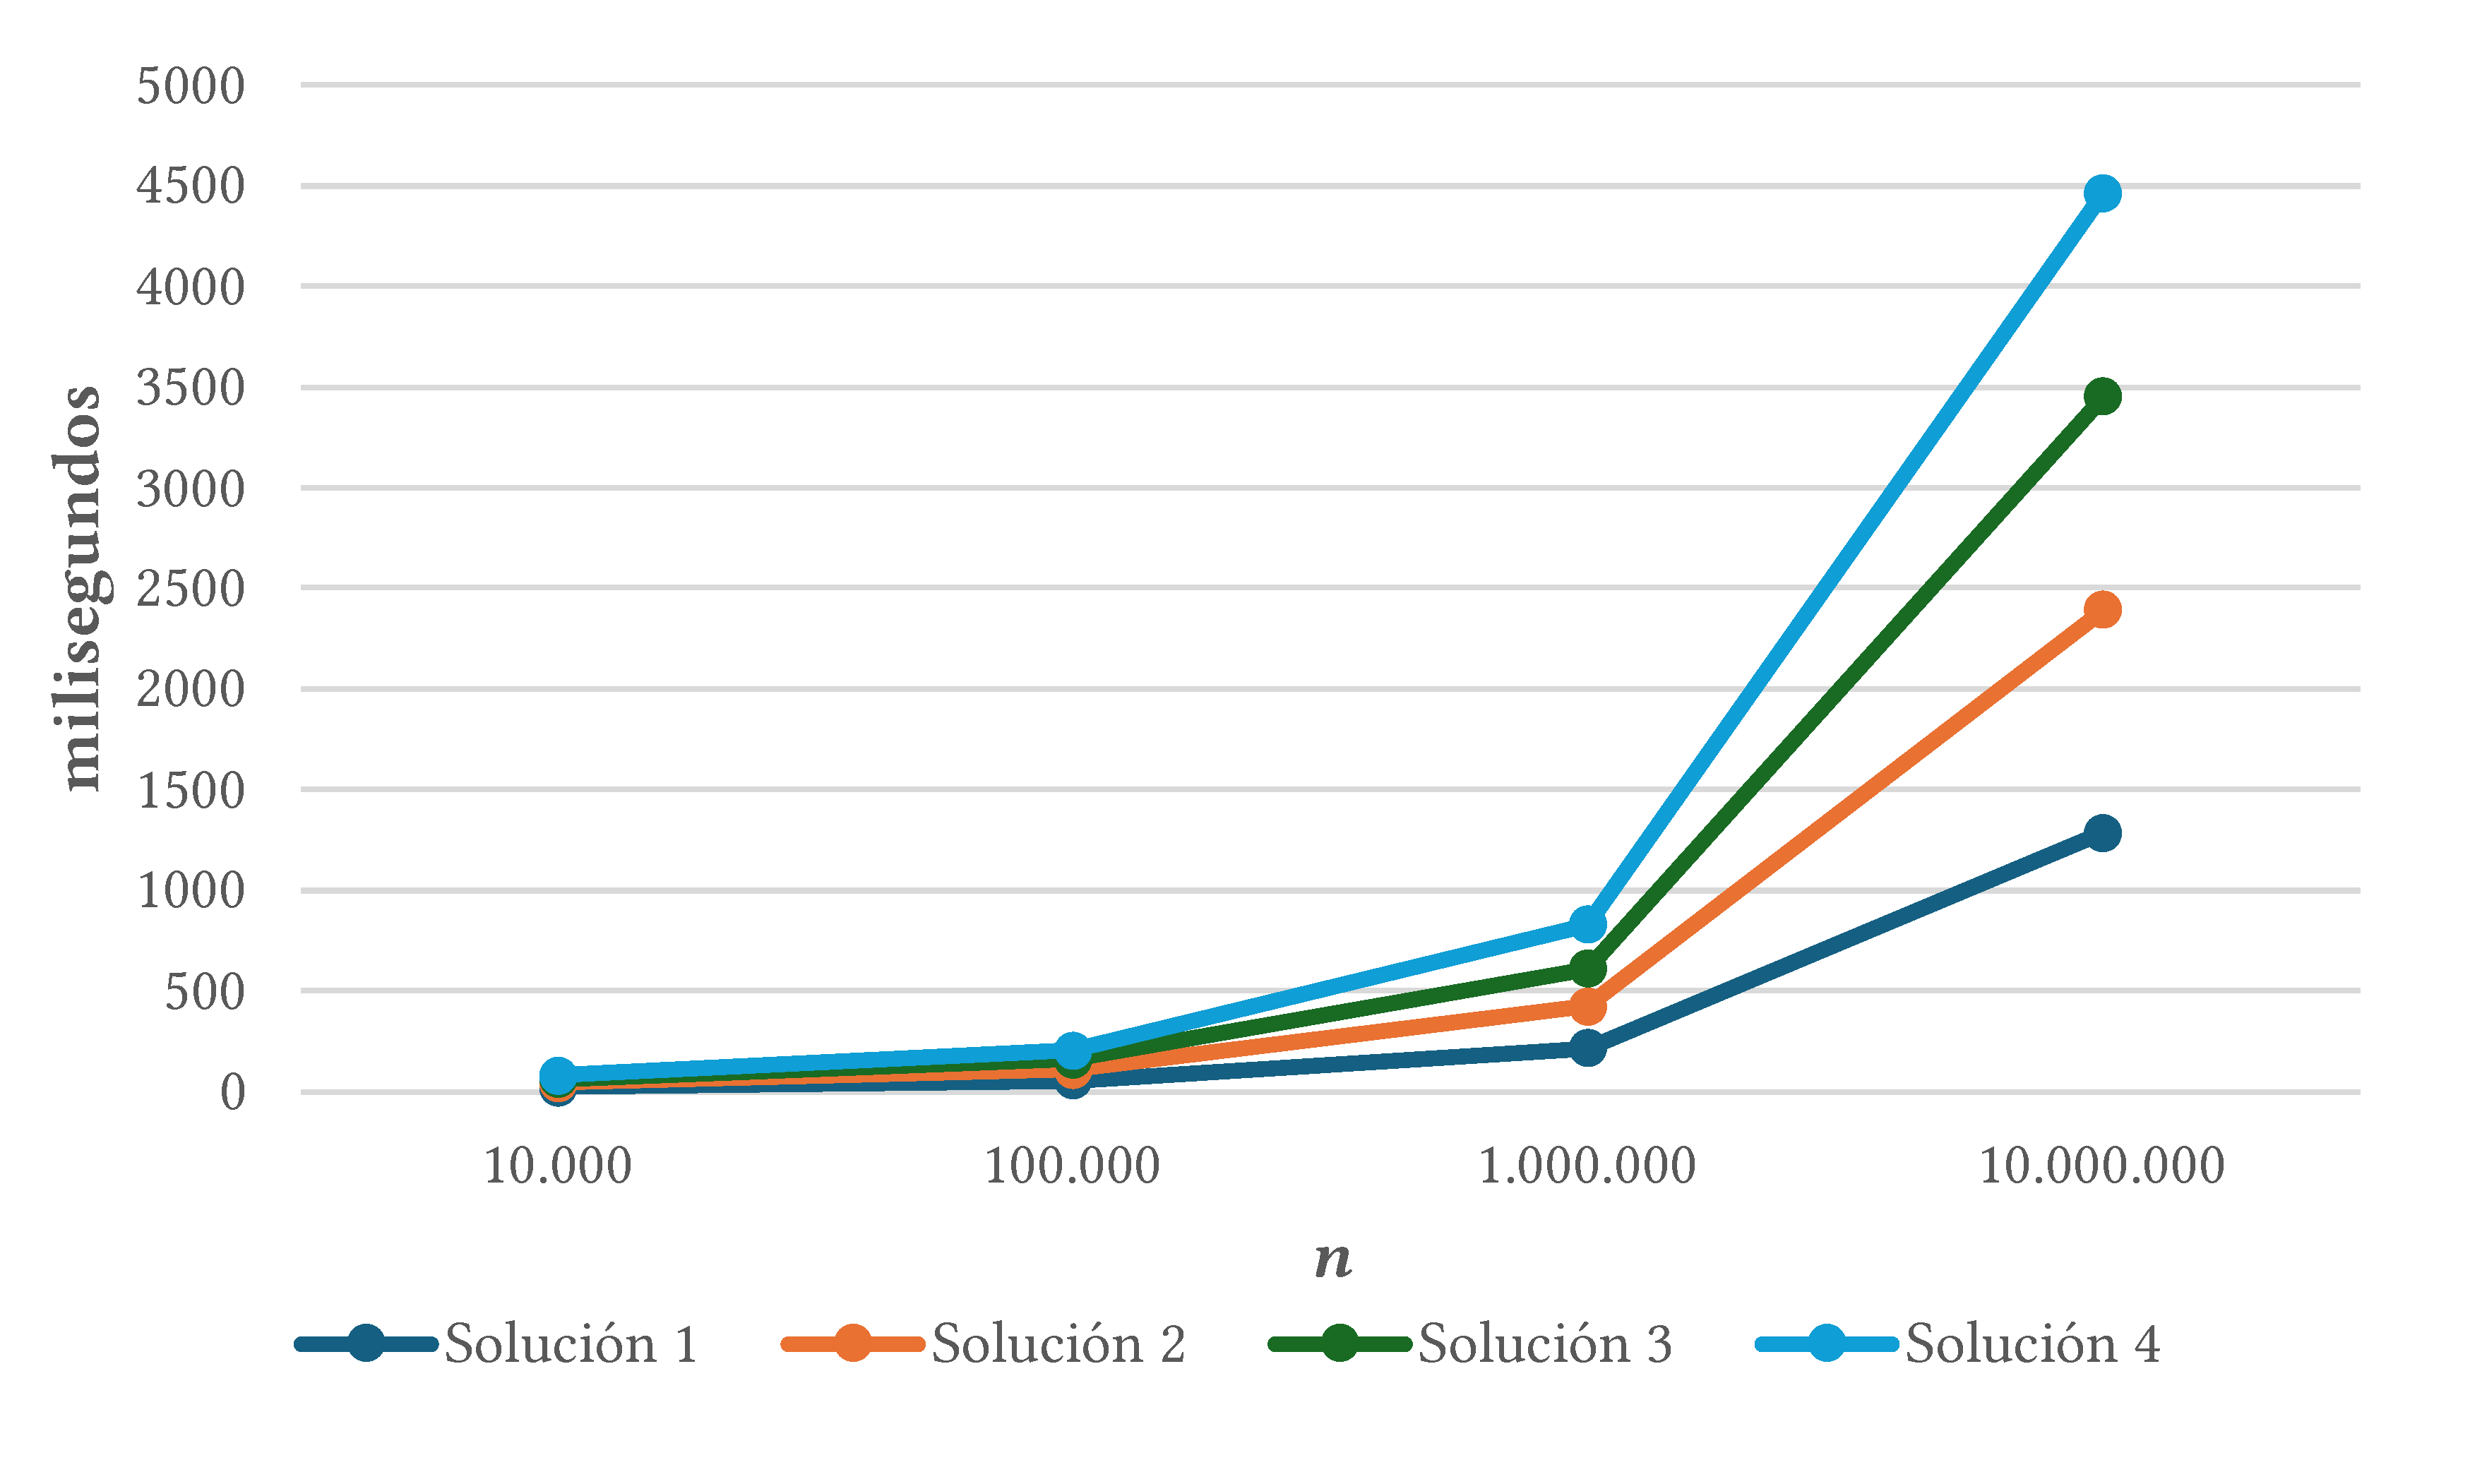
\includegraphics[width=0.78\linewidth]{../resources/practica5/images/tiempos.pdf}
\caption{Comparación de tiempos de ejecución de las cuatro implementaciones.}\label{fig-p5-tiempos}
\end{figure}

\begin{PracticeWarningBox}{Posible falta de memoria}
Para valores de \(n\) muy grandes, es posible que el programa no tenga suficiente memoria para ejecutar la criba de Eratóstenes, especialmente en las implementaciones que utilizan un vector de enteros. En ese caso, puedes aumentar la memoria asignada a Java desde \texttt{Run > Run Configurations...}, pestaña \texttt{Arguments}, añadiendo \texttt{-Xmx4g} en \texttt{VM arguments}.
\end{PracticeWarningBox}

\subsection{Medición de tiempo de ejecución}\label{medicion-de-tiempo-de-ejecucion}

Para medir el tiempo de ejecución de cada implementación, puedes utilizar la clase \texttt{System} de Java para obtener el tiempo antes y después de ejecutar el algoritmo:

\PracticeCode{../resources/practica5/snippets/java/timing.java}

\section{Solución 1: implementación básica}\label{solucion-1-implementacion-basica}

En esta implementación se utiliza un \textbf{vector de números enteros para representar los números desde 0 hasta \(n\)}, donde cada posición indica si el número correspondiente es primo o no. Un número será primo si su posición en el vector no es cero, sino igual a su propio valor.

\[
numero[i] =
\begin{cases}
i & \text{si } i \text{ es primo}\\
0 & \text{si } i \text{ no es primo}
\end{cases}
\]

\PracticeCode{../resources/practica5/snippets/java/solucion1.java}

\begin{PracticeNoteBox}{Tamaño del vector}
Cada entero ocupa 4 bytes en Java, por lo que el vector utilizado para la criba ocupará \(4(n+1)\) bytes. Por ejemplo, si \(n=100\), el vector ocupará \(4(100+1)=404\) bytes.
\end{PracticeNoteBox}

\section{Solución 2: optimización con la raíz cuadrada}\label{solucion-2-optimizacion-con-la-raiz-cuadrada}

En la solución previa se itera hasta \(n\), lo cual es ineficiente. En esta solución se optimiza el proceso iterando solo hasta la raíz cuadrada de \(n\).

\begin{PracticeWarningBox}{Optimización con la raíz cuadrada}
Si un número \(n\) no es primo, uno de sus factores \(d\) cumple \(1 \le d \le \sqrt{n}\). Si no tiene factores en ese rango, entonces es primo. Por tanto, basta con probar divisores hasta \(\sqrt{n}\).
\end{PracticeWarningBox}

\PracticeCode{../resources/practica5/snippets/java/solucion2.java}

\begin{PracticeNoteBox}{Tamaño del vector}
El vector sigue ocupando \(4(n+1)\) bytes, porque continúa usando enteros. La mejora aparece en el número de iteraciones necesarias para marcar múltiplos.
\end{PracticeNoteBox}

\section{Solución 3: vector de booleanos}\label{solucion-3-vector-de-booleanos}

En esta implementación se utiliza un \textbf{vector de booleanos} para representar si cada número es primo o no. El vector se inicializa con \texttt{true} para todos los números desde 2 hasta \(n\), y luego se marcan como \texttt{false} los múltiplos de cada número primo encontrado.

\PracticeCode{../resources/practica5/snippets/java/solucion3.java}

\begin{PracticeNoteBox}{Tamaño del vector}
El vector utilizado ocupará aproximadamente \(1(n+1)\) bytes, ya que se utiliza un booleano por cada número.
\end{PracticeNoteBox}

\section{Solución 4: solo números impares}\label{solucion-4-solo-numeros-impares}

En esta implementación se utiliza un \textbf{vector de booleanos} para representar si cada número \textbf{impar} es primo o no. Como el único número par primo es el 2, podemos ignorar los pares mayores que 2 y reducir a la mitad el tamaño del vector.

Los números impares mayores que 2 pueden escribirse como:

\[
p = 2i + 3 \quad \text{con } i = 0, 1, 2, \ldots, \left\lfloor\frac{n-3}{2}\right\rfloor
\]

Por tanto, el vector solo necesita:

\[
\left\lfloor\frac{n-3}{2}\right\rfloor + 1
\]

posiciones. Para cada primo \(p\), eliminamos sus múltiplos impares menores que \(n\): \(3p, 5p, 7p,\ldots\).

\PracticeCode{../resources/practica5/snippets/java/solucion4-template.java}

\begin{PracticeNoteBox}{Tamaño del vector}
El vector utilizado ocupará aproximadamente \(1\left(\left\lfloor(n-3)/2\right\rfloor+1\right)\) bytes. Para \(n=100\), son 49 bytes, aproximadamente el 12\% del tamaño del vector de enteros de la primera solución.
\end{PracticeNoteBox}

\section{Entrega de la solución}\label{entrega-de-la-solucion}

\textbf{Sólo debe realizar la entrega un miembro del grupo.} Sube a Moodle un fichero comprimido en formato ZIP que contenga:

\begin{itemize}
\tightlist
\item \texttt{Solucion1.java}: implementación básica utilizando un vector de enteros.
\item \texttt{Solucion2.java}: optimización utilizando la raíz cuadrada de \(n\).
\item \texttt{Solucion3.java}: implementación utilizando un vector de booleanos.
\item \texttt{Solucion4.java}: implementación con vector de booleanos y solo números impares.
\item \texttt{tiempos.xlsx}: fichero de Excel con los tiempos de ejecución para los valores de \(n\) indicados.
\end{itemize}

\end{document}
